\documentclass{beamer}

\mode<presentation> {

% The Beamer class comes with a number of default slide themes
% which change the colors and layouts of slides. Below this is a list
% of all the themes, uncomment each in turn to see what they look like.


\usetheme{default}
%\usetheme{AnnArbor}
%\usetheme{Antibes}
%\usetheme{Bergen}
%\usetheme{Berkeley}
%\usetheme{Berlin}
%\usetheme{Boadilla}
%\usetheme{CambridgeUS}
%\usetheme{Copenhagen}
%\usetheme{Darmstadt}
%\usetheme{Dresden}
%\usetheme{Frankfurt}
%\usetheme{Goettingen}
%\usetheme{Hannover}
%\usetheme{Ilmenau}
%\usetheme{JuanLesPins}
%\usetheme{Luebeck}
%\usetheme{Madrid}
%\usetheme{Malmoe}
%\usetheme{Marburg}
%\usetheme{Montpellier}
%\usetheme{PaloAlto}
%\usetheme{Pittsburgh}
%\usetheme{Rochester}
%\usetheme{Singapore}
%\usetheme{Szeged}
%\usetheme{Warsaw}

% As well as themes, the Beamer class has a number of color themes
% for any slide theme. Uncomment each of these in turn to see how it
% changes the colors of your current slide theme.

%\usecolortheme{albatross}
%\usecolortheme{beaver}
%\usecolortheme{beetle}
%\usecolortheme{crane}
%\usecolortheme{dolphin}
%\usecolortheme{dove}
%\usecolortheme{fly}
%\usecolortheme{lily}
%\usecolortheme{orchid}
%\usecolortheme{rose}
%\usecolortheme{seagull}
%\usecolortheme{seahorse}
%\usecolortheme{whale}
%\usecolortheme{wolverine}

%\setbeamertemplate{footline} % To remove the footer line in all slides uncomment this line
\setbeamertemplate{footline}[page number] % To replace the footer line in all slides with a simple slide count uncomment this line

\setbeamertemplate{navigation symbols}{} % To remove the navigation symbols from the bottom of all slides uncomment this line
}

\usepackage{graphicx}
\usepackage{amssymb}
\usepackage{color}
\usepackage{subfig}


%\AtBeginSection[]{
%  \begin{frame}
%  \vfill
%  \centering
%  \begin{beamercolorbox}[sep=8pt,center,shadow=true,rounded=true]{title}
%    \usebeamerfont{title}\insertsectionhead\par%
%  \end{beamercolorbox}
%  \vfill
%  \end{frame}
%}


\title{Image Inpainting Software}

\author{Team 27: Yesheng Ma\\\hspace{0.9cm}Hu Hu\\\hspace{1.4cm}Yikai Zou}
\institute[SJTU]{}
\date{\today}


\begin{document}
\begin{frame}
\titlepage
\end{frame}



\section{Introduction}
\begin{frame}{What is Image Inpainting?}
\begin{definition}[Inpainting]
The technique of modifying an image in an undetectable form.
\end{definition}
\begin{itemize}
\item the restoration of old photographs and damaged film
\item the removal of unwanted text
\item the removal of objects in purpose
\end{itemize}

\begin{figure}
  \centering
  \subfloat[Unwanted Text]{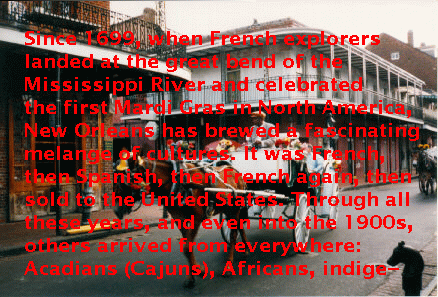
\includegraphics[height=2cm,width=3cm]{text.png}}\qquad
  \subfloat[Resotration]{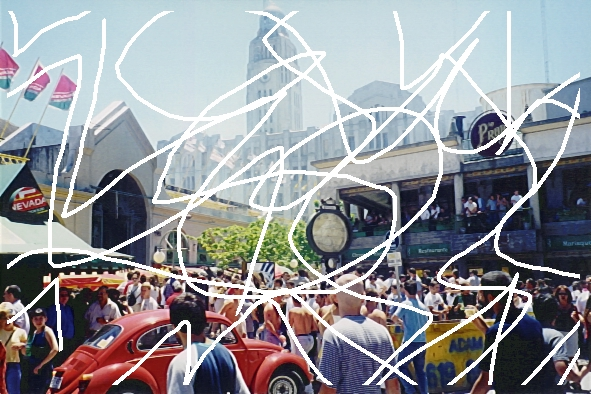
\includegraphics[height=2cm,width=3cm]{damaged.png}}
\end{figure}
\end{frame}

\section{Existing Approaches}
\begin{frame}{Existing Approaches: \emph{SIGGRAPH '00}}
The main idea is:
\begin{center}
\hspace*{-2cm}
\emph{Propagate} in the direction as the normal around \\\hspace*{-2cm}the boundary of the region to be inpainted.
\end{center}
\vspace*{-2cm}
\hspace*{8.5cm}
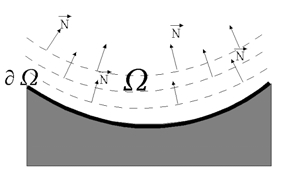
\includegraphics[height=2cm, width=3cm]{prop.png}
\pause
\vspace*{1cm}
Problems:
\begin{itemize}
\item Only local information are used.
\item How much to propagate?
\end{itemize}

\end{frame}



\section{Proposed Ideas and Implementation}
\subsection{Markov Random Field}
\begin{frame}{Markov Random Field}
Model the image as a Markov random field:\\
\quad make use the image structure!


\hspace*{8cm}
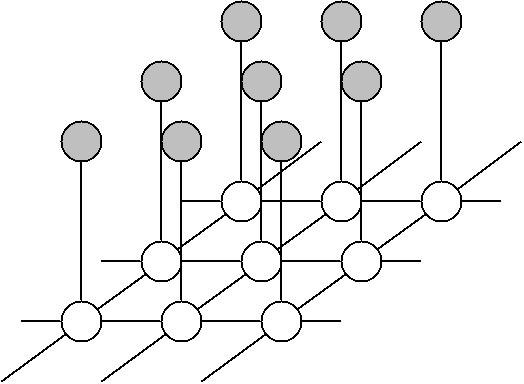
\includegraphics[height=2cm, width=3cm]{mrf.jpg}

\vspace*{-1cm}
\begin{enumerate}
\item Create a model with image prior.
\item Train that model with a dataset.
\item Propagate information with that learned model.
\end{enumerate}
\end{frame}

\begin{frame}{Implementation of MRF}
\begin{enumerate}
\item Implement the MRF model in MATLAB (useful toolboxes!)
\item About model: a technique of \emph{product of experts} by Hinton
\item About training: perform a gradient ascent
\item About dataset: Berkeley dataset with 500 inpainting images
\end{enumerate}
\end{frame}

\subsection{Exemplar-Based Algorithm}
\begin{frame}{Exemplar-Based Algorithm}
	\textbf{Observations:}
	\begin{itemize}[<+->]
		\item Using single pix as basic unit will result in blurry. \\So we using patch (i.e. 3x3) as basic unit.
		\item In-painting order is important for final result. 
		\begin{figure}
			\centering
			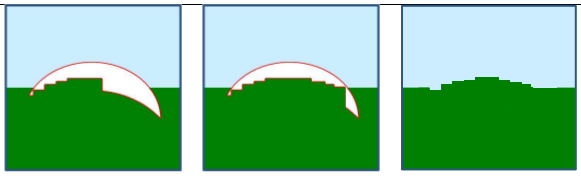
\includegraphics[width=0.8\linewidth]{order1.png}\\
			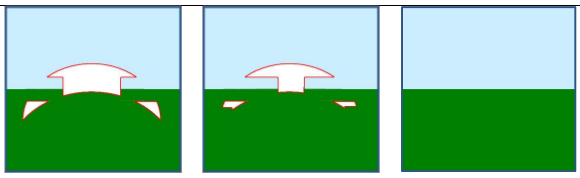
\includegraphics[width=0.8\linewidth]{order2.png}
			\caption{In-painting by different order}
		\end{figure}
	\end{itemize}
\end{frame}
%
\begin{frame}{Exemplar-Based Algorithm}
	\textbf{In-painting Process:}
	\begin{itemize}[<+->]
		\item Patch selection: We need to select the specific patch to inpaint first. We define the priority function:
		\begin{equation*}
		\centering
		P(p)=C(p)*D(p)
		\nonumber
		\end{equation*}
		where: $C(p)=\frac{\sum_{q\in \Phi _p\cap(-\Omega)}*C(q)}{|\Phi_p|}$, $D(p)=\frac{|\nabla I^\bot_p \cdot n_p|}{\alpha}$.
		\item During each loop, we calculate the C(p) and D(p) of each patch, choose the patch with maximum priority.
		\item Then we find the exemplar patch that minimize the Euclidean distance between them and inpaint the former patch.
		\item We implemented this algorithm in python.
	\end{itemize}
\end{frame}


\section{Demo}
\begin{frame}{Demo}
	\begin{itemize}
		\item Using Markov random field algorithm:
		\begin{figure}
			\centering
			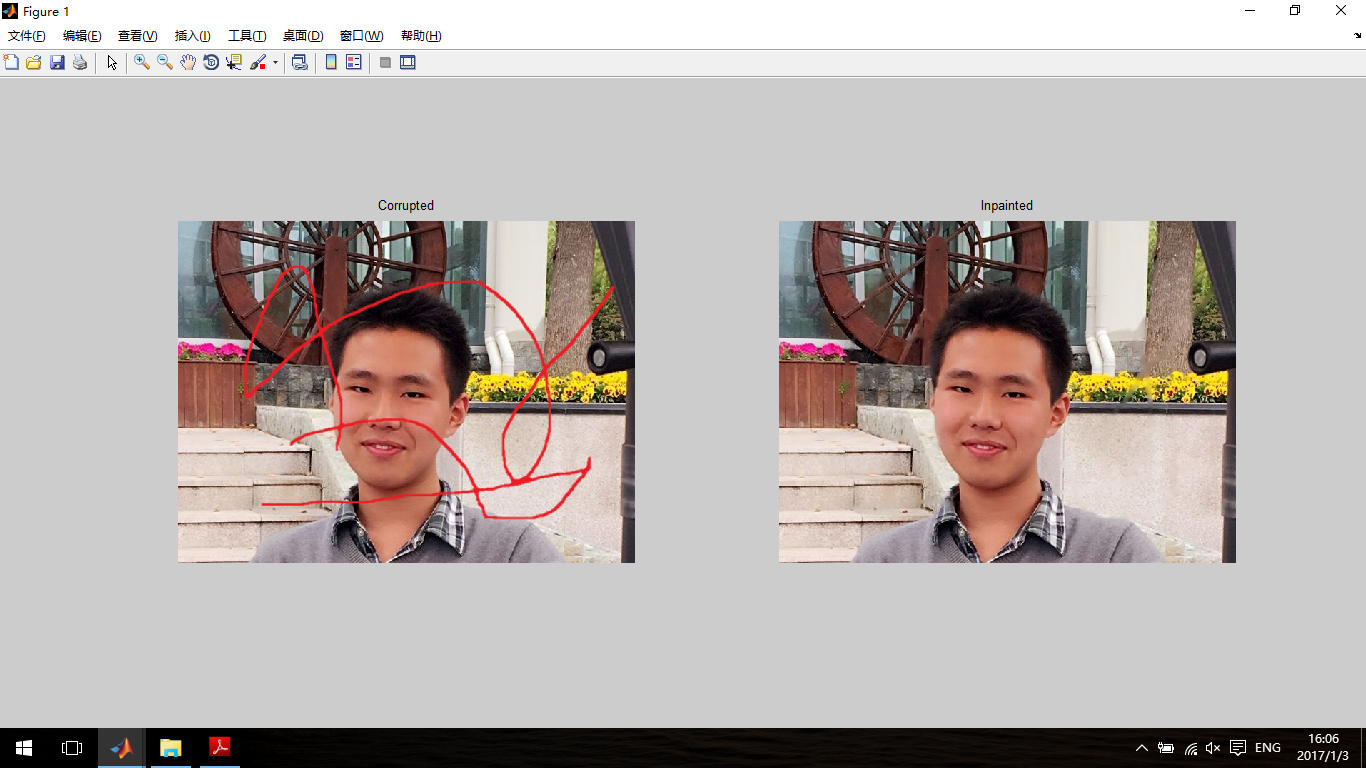
\includegraphics[width=1.0\linewidth]{rmf_result.png}
			\caption{Result by MRF Implementation}
		\end{figure}
	\end{itemize}
\end{frame}

\begin{frame}{Demo}
	\begin{itemize}
		\item Using exemplar-based algorithm:
		\begin{figure}
			\centering
			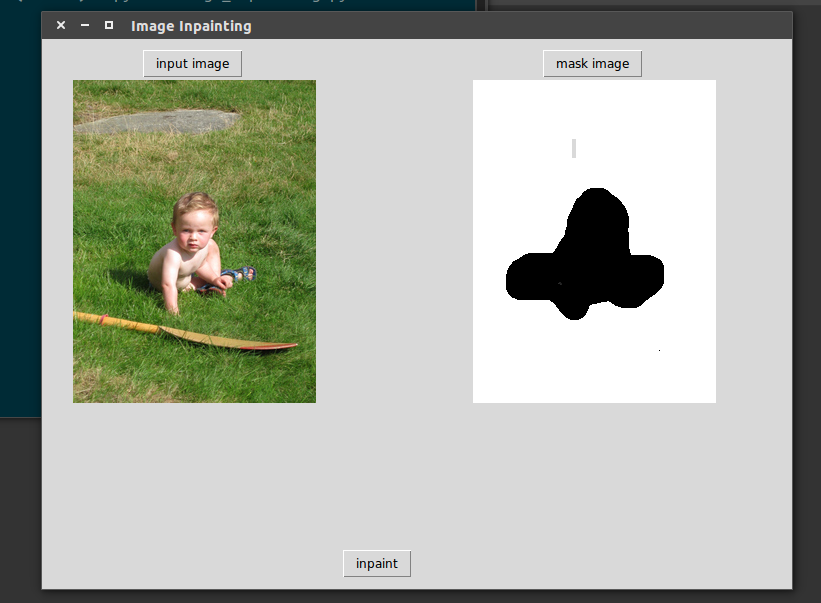
\includegraphics[width=0.8\linewidth]{eb_result.png}
			\caption{Result by exemplar-based Implementation}
		\end{figure}
	\end{itemize}
\end{frame}

\begin{frame}{Demo: using exemplar-based algorithm (Cont'd)}
		\begin{figure}
		  \centering
		  \subfloat[Original picture]{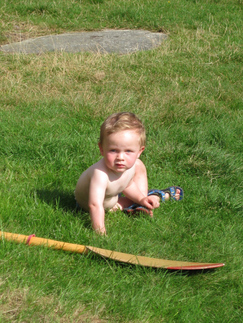
\includegraphics[height=5cm,width=4.5cm]{in1.jpg}}\qquad
		  \subfloat[In-painted picture]{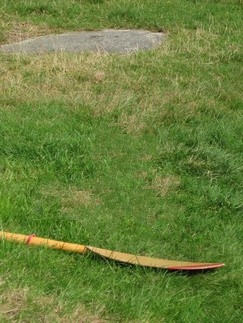
\includegraphics[height=5cm,width=4.5cm]{out1.jpg}}
		\caption{Result by exemplar-based Implementation}
		\end{figure}
\end{frame}


\section{Conclusion and Future Work}
\begin{frame}{Conclusion and Future Work}
	\begin{itemize}[<+->]
		\item We accomplished the chosen task and solved the problem. The result works well.
		\item The proposed ideas given by us successfully solve the Image In-painting problem.\\\ \\ 
		\item In this AI age, we plan to apply deep learning model in this topic in the future. We have designed the network structure for image in-painting. If we get enough data one day, we will try this deep learning model on this topic.
	\end{itemize}
\end{frame}
%
\section*{Reference}
\begin{frame}{Reference}
	\begin{itemize}
		\item M. Bertalmio, G. Sapiro, V. Caselles, and C. Ballester, Image in-painting, in $Proc.\ SIGGRAPH$, 2000, pp. 417-424
		\item S. Roth and M. J. Black. Fields of experts. $IJCV$, 82(2):205–229,
		2009.
		\item A. Criminisi, P. Perez, and K. Toyama, Region filling and object
		removal by examplar-based image inpainting, IEEE $Trans. Image\ 
		Process.$, vol. 13, pp. 1200-1212, 2004.
		\item G. E. Hinton. Training products of experts by minimizing contrastive
		divergence. $Neural\ Comput.$, 14(8):1771-1800, 2002.
		\item M. Welling, G. E. Hinton, and S. Osindero. Learning sparse topographic representations with products of Student-t distributions.
		$NIPS*2002$.
	\end{itemize}
\end{frame}

\begin{frame}
\centering
\Huge{{The End}}
\end{frame}
\end{document}
